\chapter{The RoboCup Competition}
\label{background}

RoboCup is an international robotics competition founded in 1997. The aim is to promote robotics, artificial intelligence, and machine learning research by offering a publicly appealing, but formidable, challenge. The name \textit{RoboCup} is a contraction of the competition's full name, ``Robot Soccer World Cup''. The official goal of the project is stated as an ambitious endeavor: ``By the year 2050, a team of fully autonomous humanoid robot soccer players shall win the soccer game, complying with the official rule of the FIFA, against the winner of the most recent World Cup''~\cite{robocup}. This endeavor may seem impossible with today's technology. I would say that a more realistic goal would be to make a team of robots play soccer similarly, but not necessarily better, than humans. In any case, the true goal is to push research efforts towards technological breakthroughs and will be the one of the grand challenges shared by robotics and AI community for next 50 years. RoboCup is an annual event in which lots of research teams around the world participate in various leagues including RoboCupSoccer, RoboCup@Home, RoboCupRescue, and RoboCupJunior, each of these leagues and its sub-leagues will be presented extensively below. Participation in this annual event is growing year by year reaching in a number of more than 400 teams from 40 countries around the world in RoboCup 2011 which held in Istanbul, Turkey. The RoboCup competitions provide an excellent channel for the dissemination and validation of innovative concepts and approaches for autonomous robots and multi-robot systems under very challenging and adverse conditions.


\section{RoboCup Soccer}

The main focus of the RoboCup competitions is the game of soccer, where the research goals concern cooperative multi-robot systems in dynamic adversarial environments. All robots in this league are fully autonomous. A competition which gives the possibility of doing research in a more entertaining way. Moreover, we can realize that soccer is selected due to the fact that it is a popular sport and widely spread throughout the world. Moreover, rules governing it are also known. Robocup Soccer encompasses all the known problems of artificial intelligence such as machine vision, perception, behavior and cooperation which are of paramount importance in multi-agent environments like this.


\subsubsection*{Humanoid League} 
In the Humanoid League, autonomous robots with a human-like body and human-like senses play soccer against each other. Dynamic walking, running, and kicking the ball while maintaining balance, visual perception of the ball, other players, and the field, self-localization, and team play are among the many research issues investigated in the league. The league is divided into 3 subleagues, according to robot sizes: Teen, Kid and Adult Size. Figure~\ref{fig:HumanoidCaption} shows these three size leagues.

\begin{figure}[t!] 
\centering
    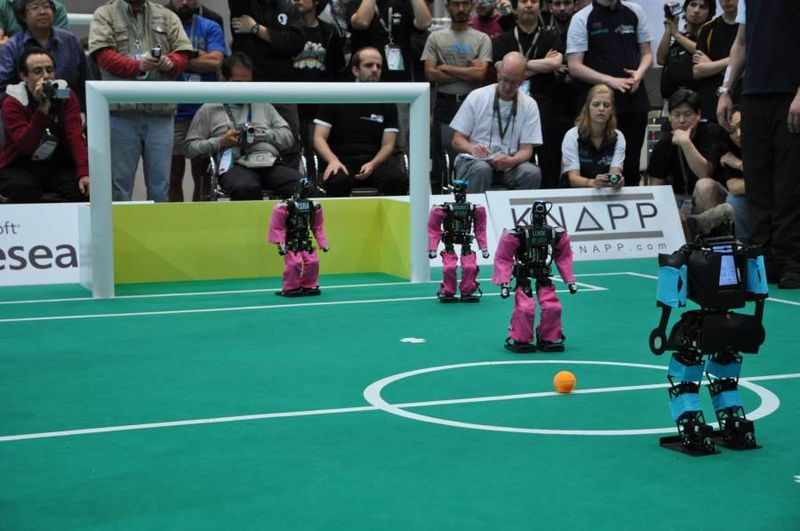
\includegraphics[height=4cm]{Chapter1/figures/kid2011.jpg}\ 
    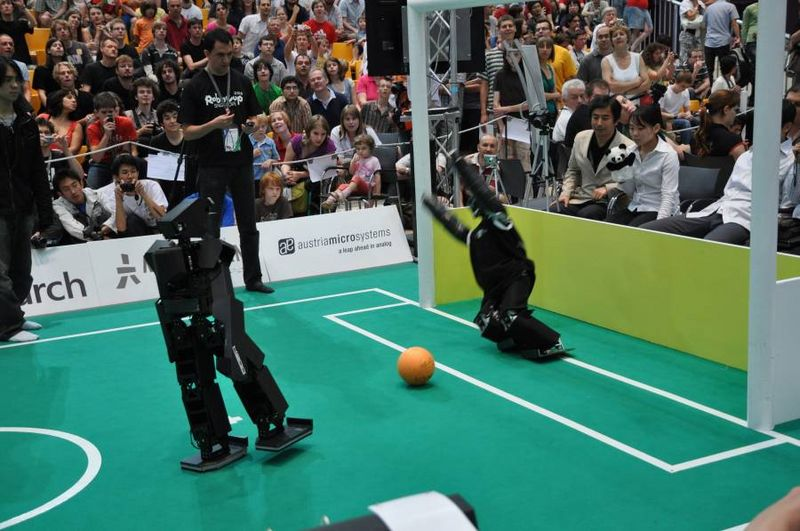
\includegraphics[height=4cm]{Chapter1/figures/teen2011.jpg}\ 
    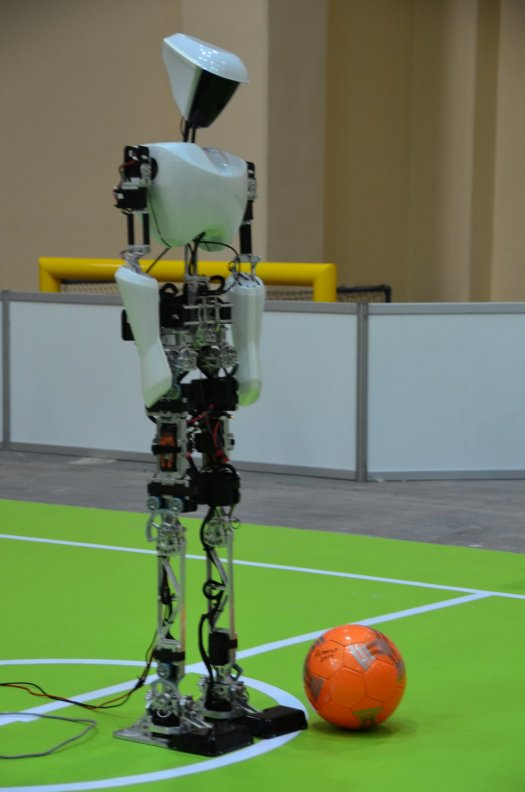
\includegraphics[height=4cm]{Chapter1/figures/adult2011.jpg}
\caption{Humanoid Kid, Teen, Adult -Size League at Robocup 2011.}
  \label{fig:HumanoidCaption}
\end{figure}

\subsubsection*{Middle-Size League}
Middle-sized wheeled robots of no more than 50 cm diameter play soccer in teams of up to six robots with regular size FIFA soccer ball on a field similar to a scaled human soccer field. All sensors are on-board. Robots can use wireless networking to communicate. The research focus is on full autonomy and cooperation at plan and perception levels. Figure~\ref{fig:Middle} shows a Middle-Size League's game at RoboCup 2011.

\begin{figure}[t!]
\centering
  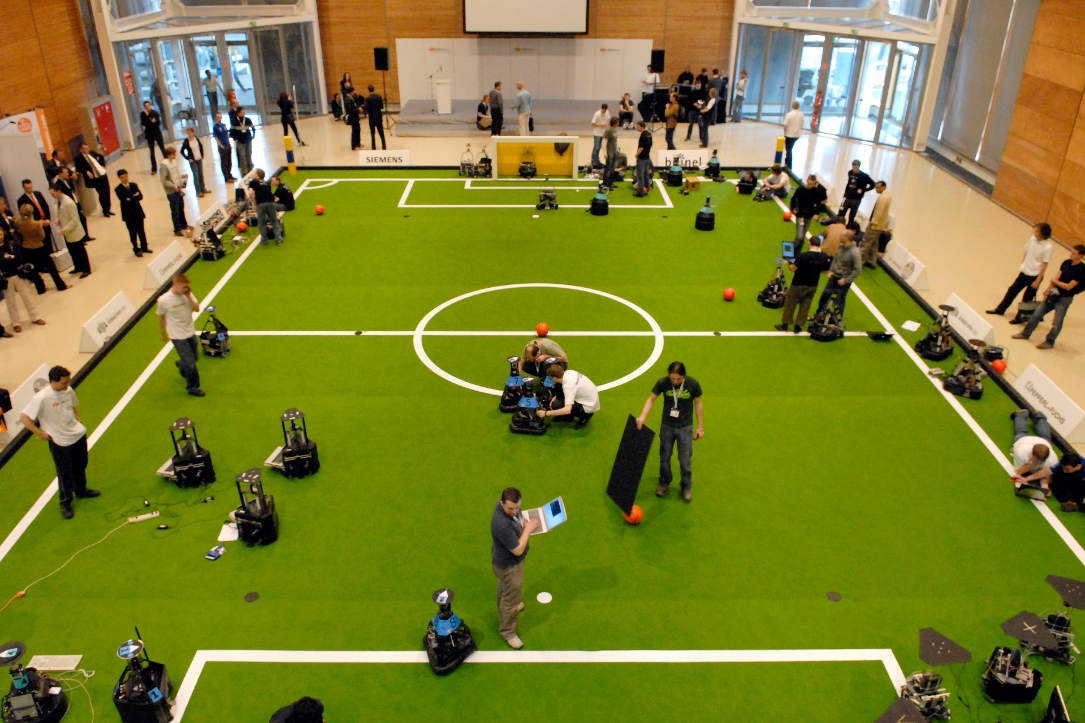
\includegraphics[width=0.8\textwidth]{Chapter1/figures/middleSize.jpg}
  \caption{Middle-Size League at RoboCup 2011.}
  \label{fig:Middle}
\end{figure}

\subsubsection*{Simulation League}
This is one of the oldest leagues in RoboCup's Soccer. The Simulation League focus on artificial intelligence and team strategy. Independently moving software players (agents) play soccer on a virtual field inside a computer. There are two subleagues: 2D and 3D. Simulation league 3D is going to be presented extensively in the next chapter. Figure~\ref{fig:sim2d3d} shows how the 2D versus 3D simulation league looks like.

\begin{figure}[t!] 
\centering
    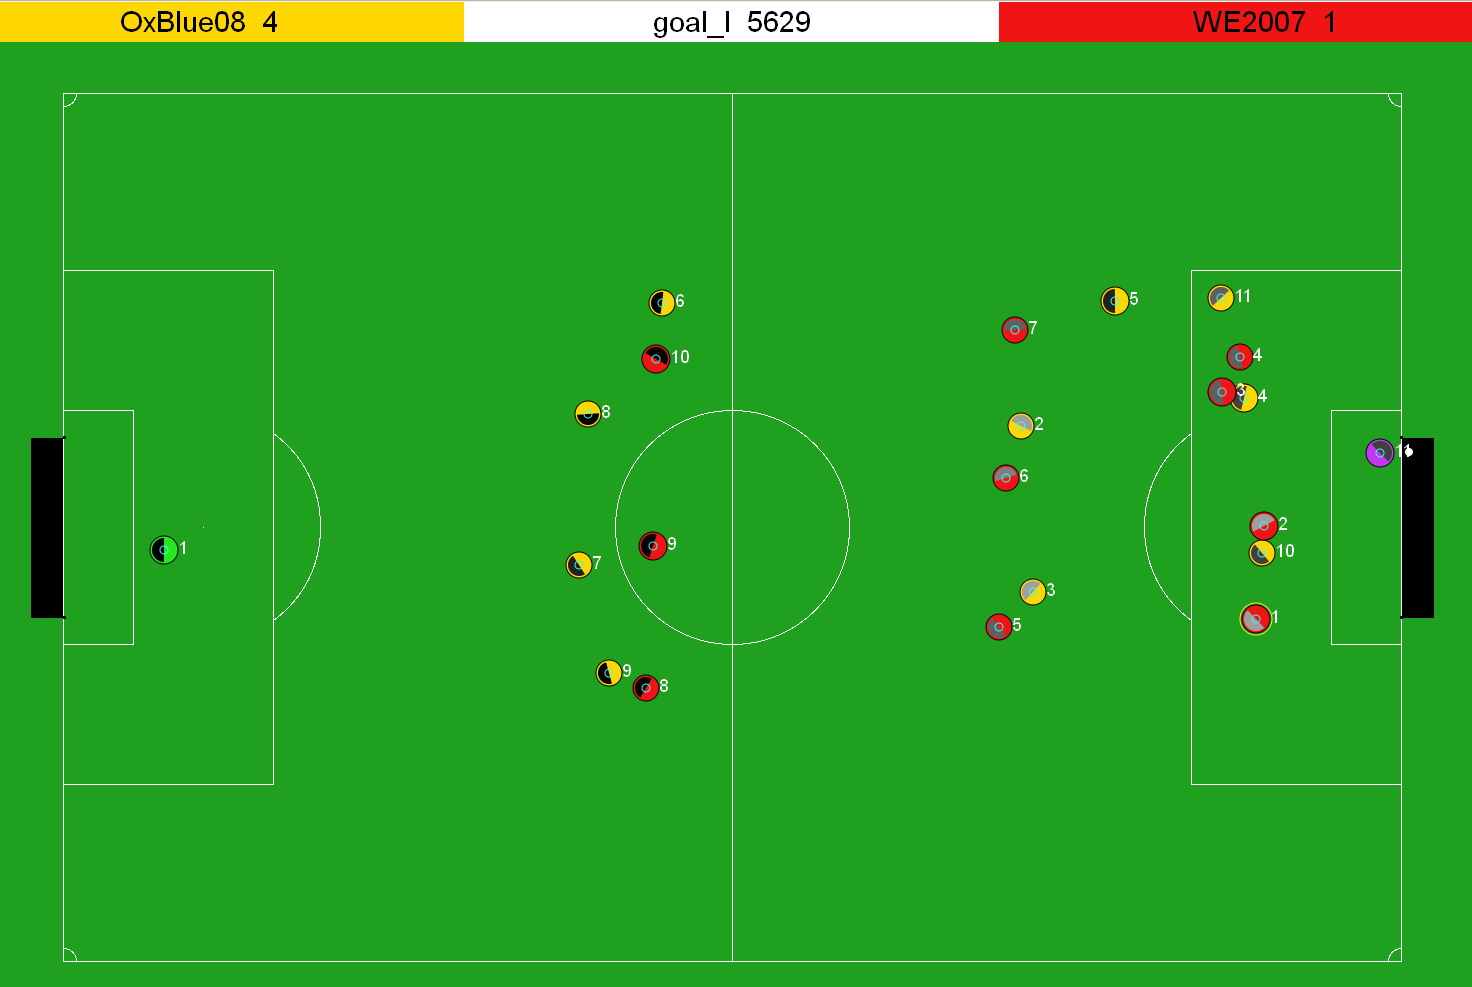
\includegraphics[height=5cm]{Chapter1/figures/2D.jpg}\ \ \ 
    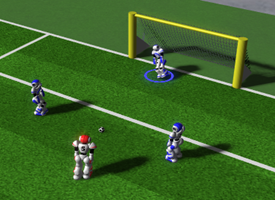
\includegraphics[height=5cm]{Chapter1/figures/3d.png}
  \caption{Simulation League 2D (left) and 3D (right).}
  \label{fig:sim2d3d}
\end{figure}

\subsubsection*{Small-Size League}
The Small Size league or F180 league as it is otherwise known, is one of the oldest RoboCup Soccer leagues. It focuses on the problem of intelligent multi-robot/agent cooperation and control in a highly dynamic environment with a hybrid centralized/distributed system. The robot must fit within an 180mm diameter circle and must be no higher than 15cm. The robots play soccer with an orange golf ball on a green carpeted field that is 6.05m long by 4.05m wide. All objects on the field are tracked by a standardized vision system that processes the data provided by two cameras that are attached to a camera bar located 4m above the playing surface. The vision system called SSL-Vision. Figure~\ref{fig:small} shows a game during RoboCup competition in Istanbul, 2011.

\begin{figure}[t!]
\centering
  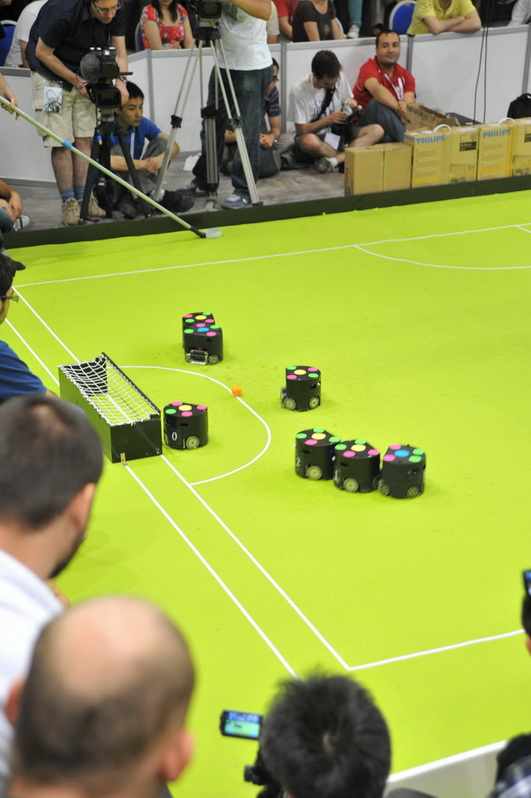
\includegraphics[trim=0cm 4cm 0cm 2cm, clip, width=0.5\textwidth]{Chapter1/figures/SmallSize.jpg}
  \caption{Small-Size League at RoboCup 2011.}
  \label{fig:small}
\end{figure}




\subsubsection*{Standard Platform League}
In this league all teams use same robots. Therefore, the teams concentrate on software development only, while still using state-of-the-art robots. Directional vision forces decision-making to trade vision resources for self-localization and ball localization. The league is based on Aldebaran�s Nao humanoids. Team ``Kouretes''  [\url{www.kouretes.gr}] from the Technical University of Crete is the only Greek representative in this league, having continuous participation since 2006 and several distinctions. Figure~\ref{fig:SPL} shows a highlight of the Standard Platform League.

\begin{figure}[t!]
\centering
  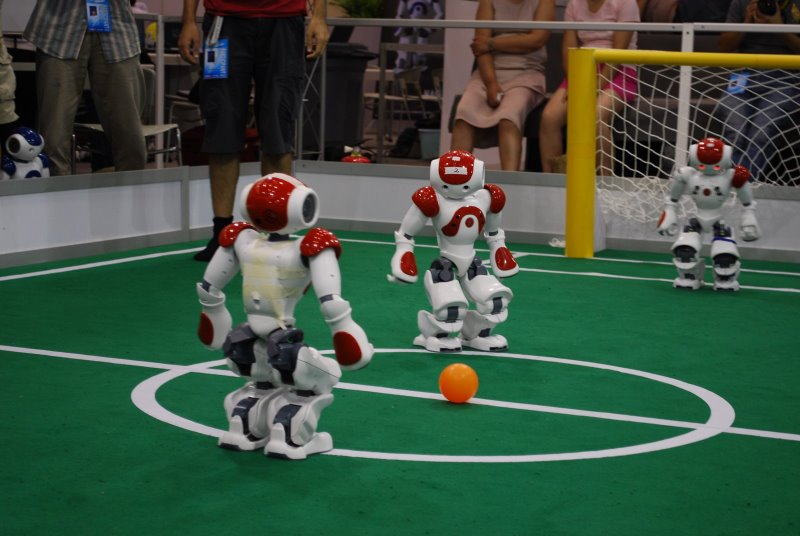
\includegraphics[width=0.8\textwidth]{Chapter1/figures/spl.jpg}
  \caption{Standard Platform League at RoboCup 2011.}
  \label{fig:SPL}
\end{figure}


\section{RoboCup Rescue}
The intention of the RoboCup Rescue project is to promote research and development in this socially significant domain at various levels involving multi-agent team work coordination, physical robotic agents for search and rescue, information infrastructures, personal digital assistants, a standard simulator and decision support systems, evaluation benchmarks for rescue strategies and robotic systems that are all integrated into a comprehensive systems in future.

\subsubsection*{Robot League}
The goal of the urban search and rescue (USAR) robot competitions is to increase awareness of the challenges involved in search and rescue applications, provide objective evaluation of robotic implementations in representative environments, and promote collaboration between researchers. It requires robots to demonstrate their capabilities in mobility, sensory perception, planning, mapping, and practical operator interfaces, while searching for simulated victims in unstructured environments. The RoboCupRescue arenas constructed to host these competitions consist of emerging standard test methods for emergency response robots developed by the U.S. National Institute of Standards and Technology through the ASTM International Committee on Homeland Security Applications; Operational Equipment; Robots (E54.08.01). The competition field is divided into color-coded arenas that form a continuum of challenges with increasing levels of difficulty for robots and operators and highlight certain robotic capabilities.
Greece participates in this league (RoboCup 2008, 2009, 2011) with team ``P.A.N.D.O.R.A'' [\url{pandora.ee.auth.gr}] based at the Aristotle University of Thessaloniki. Figure~\ref{fig:pandora} shows a wheeled robot in RoboCupRescue robot competition.

\begin{figure}[t!]
\centering
  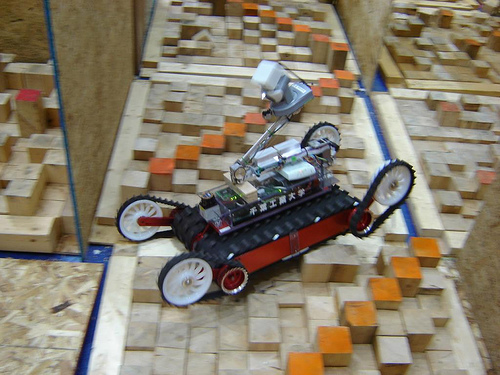
\includegraphics[width=0.6\textwidth]{Chapter1/figures/rescue.jpg}
  \caption{Rescue Robot League at RoboCup 2011.}
  \label{fig:pandora}
\end{figure}

\subsubsection*{Simulation League}
The purpose of the RoboCup Rescue Simulation league is twofold. First, it aims to develop simulators that form the infrastructure of the simulation system and emulate realistic phenomena predominant in disasters. Second, it aims to develop intelligent agents and robots that are given the capabilities of the main actors in a disaster response scenario. The Virtual Robots Competition aims to be the meeting point between researchers involved in the Agents Competition and those active in the RoboCupRescue League. 
It is based on USARSim, a high fidelity simulator based on the UnrealTournament game engine. USARSim currently features wheeled, tracked and legged robots, as well as a wide range of sensors and actuators. Moreover, users can easily develop models of new robotic platforms, sensors and test environments. Validation experiments have shown close correlation between results obtained within  USARSim and the corresponding real robots. Figure~\ref{fig:SimRescue} shows a wheeled robot in RoboCupRescue robot competition.

\begin{figure}[t!]
\centering
  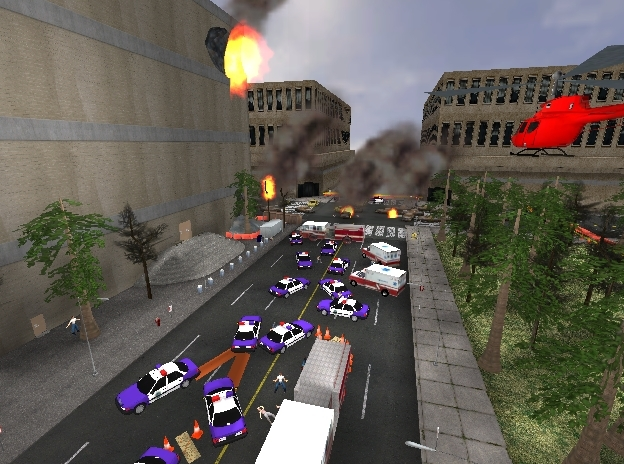
\includegraphics[width=0.8\textwidth]{Chapter1/figures/Bremen2006.jpg}
  \caption{Rescue Simulation League at RoboCup 2006.}
  \label{fig:SimRescue}
\end{figure}

\section{RoboCup@Home}

The RoboCup@Home league aims to develop service and assistive robot technology with high relevance to future personal domestic applications. It is the largest international annual competition for autonomous service robots and is part of the RoboCup initiative. A set of benchmark tests is used to evaluate the robots' abilities and performance in a realistic non-standardized home environment setting. Focus lies on, but is not limited to, the following domains: Human-Robot Interaction and Cooperation, Navigation and Mapping in Dynamic Environments, Computer Vision and Object Recognition under Natural Light Conditions, Object Manipulation, Adaptive Behaviors, Behavior Integration, Ambient Intelligence, Standardization and System Integration.

\begin{figure}[t!]
\centering
  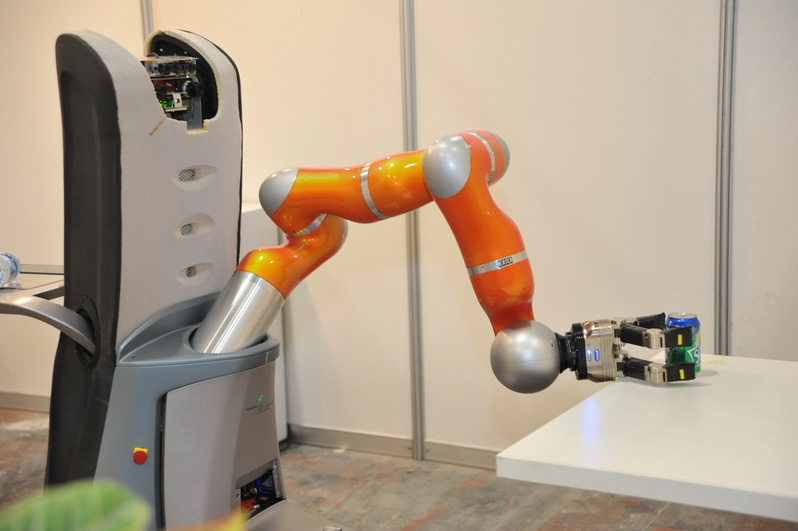
\includegraphics[width=0.8\textwidth]{Chapter1/figures/RoboCup@Home.jpg}
  \caption{RoboCup@Home at RoboCup 2011.}
  \label{fig:RoboCup@Home}
\end{figure}


\section{RoboCup Junior}

RoboCupJunior is a project-oriented educational initiative that sponsors local, regional and international robotic events for young students. It is designed to introduce RoboCup to primary and secondary school children, as well as undergraduates who do not have the resources to get involved in the senior leagues yet. 

\subsubsection*{Soccer}
2-on-2 teams of autonomous mobile robots play in a dynamic environment, tracking a special light-emitting ball in an enclosed, landmarked field. Figure~\ref{fig:Junior} shows Junior Soccer League at RoboCup 2011.

\subsubsection*{Dance}
One or more robots join human dancers and give a dance performance dressed in costume and moving in creative harmony.

\subsubsection*{Rescue}
Robots identify simulated victims within re-created disaster scenarios, varying in complexity from line-following on a flat surface to negotiating paths through obstacles on uneven terrain.

\begin{figure}[t!]
\centering
  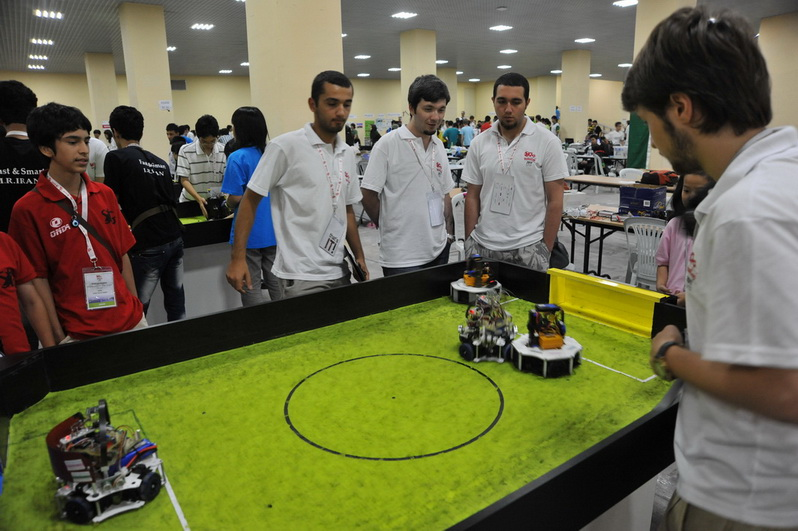
\includegraphics[width=0.8\textwidth]{Chapter1/figures/JuniorSoccer.jpg}
  \caption{Junior Soccer League at RoboCup 2011.}
  \label{fig:Junior}
\end{figure}